Ein Flugzeug fliegt auf einer Höhe von \hfO\ mit einer Geschwindigkeit von \vflO\ direkt über einen Schiffbrüchigen hinweg.

\begin{center}
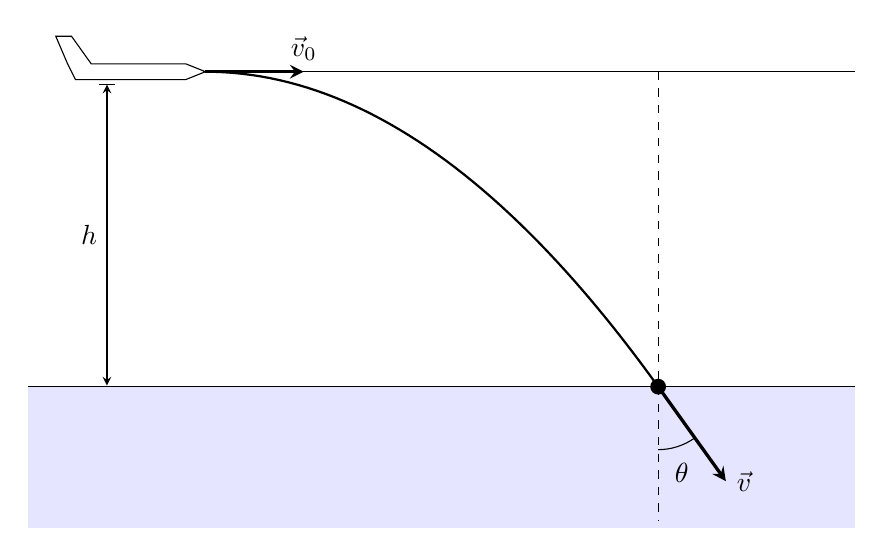
\begin{tikzpicture}[>=stealth]
 \fill[blue!10] (-2,0) rectangle (8.5,-1.8);
 \draw (-2,0) -- (8.5,0);
 \draw (-1.4,3.9) -- (0,3.9) -- (0.25,4) -- (0,4.1) -- (-1.2,4.1) -- (-1.45,4.45) -- (-1.65,4.45) -- (-1.5,4.1) -- cycle;
 \draw (0.25,4) -- (8.5,4);
 \draw[->, very thick] (0.25,4) -- (1.5,4) node[above] {$\vec v_0$};
 \draw[thick, domain=0.25:6, samples=50] plot (\x, {4-4*((\x-0.25)/5.75)^2});
 \draw[dashed] (6,4) -- (6,-1.7);
 \fill (6,0) circle (0.1);
 \draw[->, very thick] (6,0) -- (6.86,-1.2) node[right] {$\vec v$};
 \draw (6,-0.8) arc[start angle=270, end angle=305.7, radius=0.8];
 \node at (6.3,-1.1) {$\theta$};
 \draw[|<->|] (-1.0,0) -- (-1.0,3.85) node[midway, left] {$h$};
\end{tikzpicture}
\end{center}

\begin{abcliste}
\abc Wie lange ist die Rettungskapsel in der Luft?
\abc Wo muss der Pilot die Rettungskapsel fallen lassen, damit diese bei der Person im Wasser landet?
\abc Mit welcher Geschwindigkeit (Betrag und Richtung) fällt die Rettungskapsel ins Wasser?
\end{abcliste}
